\documentclass[../mathNotesPreamble]{subfiles}

\begin{document}
%  \relscale{1.4} %TODO
  \section{6.1: Probability Distributions Are Models of Random Experiments}
    \begin{defn*}
      The \textbf{probability distribution} describes
      \begin{itemize}
        \item all possible outcomes of a random experiment, and
        \item the probability of each outcome.
      \end{itemize}
      This is sometimes also referred to as the \textbf{probability distribution function (pdf)}.
    \end{defn*}
    
    \begin{ex*}
      Suppose we are reading Amazon reviews of a particular product. In total, the product has $3,901$ reviews, distributed as shown below.
    \end{ex*}
    
    \begin{center}
      \begin{minipage}{0.2\linewidth}
        \begin{tabular}{@{}cc@{}}\toprule
          Stars& Frequency\\\midrule
          5 & 0.44\\
          4 & 0.15\\
          3 & 0.10\\
          2 & 0.11\\
          1 & 0.20\\\bottomrule
        \end{tabular}
      \end{minipage}\hspace*{15mm}%
      \begin{minipage}{0.425\linewidth}
        \begin{tikzpicture}
          \begin{axis}[
            axis lines=center,
            axis line style={black,->},
            xmin=0.65, xmax=5.35,
            ymin=0,
            xlabel=Stars, xlabel style={at={(axis description cs:0.5,-0.05)},anchor=north},
            ylabel=Frequency, ylabel style={at={(axis description cs:-0.1, 0.5)},rotate=90, anchor=south},
            ticklabel style={font=\normalsize,inner sep=0.5pt,fill=white,opacity=1.0, text opacity=1}]
            \foreach \star/\freq in {
              5/0.44,
              4/0.15,
              3/0.10,
              2/0.11,
              1/0.20
              }{
                \addplot[draw=lander_blue, line width=0.95pt] coordinates{(\star,0) (\star,\freq)};
                \addplot[soldot, mark size=2pt, lander_blue] coordinates{(\star,\freq)};
              }
          \end{axis}
        \end{tikzpicture}
      \end{minipage}
    \end{center}
    
    \noindent
    \begin{extasks}[after-item-skip=\stretch{1}](1)
      \task If we pick a reviewer at random, what is the probability that they give a 5 star review? What about a 1 star review?
      \task What is the sum of the probabilities?
    \end{extasks}
  \vspace*{\stretch{1}}
  \pagebreak
  
  \begin{center}
    \fbox{\parbox{0.5\linewidth}{
      \emph{Note}: Valid probability distributions:
      \begin{itemize}
        \item Have probabilities between 0 and 1,
        \item The sum of the probabilities is \emph{exactly} 1.
      \end{itemize}
    }}
  \end{center}
  \vspace*{1\baselineskip}
  
  \begin{ex*}
    Suppose a couple decides they will keep having children until they have a girl. Assuming that the likelihood of having a boy or girl is equally likely, the probability of having $x$ children can be given by $\parens{1/2}^x$, and is represented by the graph below.
  \end{ex*}
  \begin{center}
    \begin{tikzpicture}[declare function={
      f(\x)=2^(-\x);}]
      \begin{axis}[
        axis lines=center,
        axis line style={black,->},
        xmin=0.65, xmax=10.35,
        ymin=0, ymax=0.525,
        xlabel=Number of Children until a Girl, xlabel style={at={(axis description cs:0.5,-0.05)},anchor=north},
        ylabel=Probability, ylabel style={at={(axis description cs:-0.1, 0.5)},rotate=90, anchor=south},
        ticklabel style={font=\normalsize,inner sep=0.5pt,fill=white,opacity=1.0, text opacity=1}]
        \foreach \numKids in {1,...,10}{
          \addplot[draw=lander_blue, line width=0.95pt] coordinates{(\numKids,0) (\numKids,{f(\numKids)})};
          \addplot[soldot, mark size=2pt, lander_blue] coordinates{(\numKids,{f(\numKids)})};
          }
      \end{axis}
    \end{tikzpicture}
  \end{center}
  
  \begin{extasks}[after-item-skip=\stretch{1}](1)
    \task What is the maximum number of children possible?
    \task Do the probabilities sum to 1?
  \end{extasks}
  \vspace*{\stretch{1}}
  \pagebreak

  \begin{center}
    \fbox{\parbox{0.6\linewidth}{
      Finding the probabilities for continuous outcomes:
      \begin{itemize}
        \item is represented as area under a curve,
        \item is in the context of a range of values, and
        \item the probability of hitting an exact value is 0
      \end{itemize}
    }}
  \end{center}
  \vspace*{2\baselineskip}
  
  \begin{ex*}
    Suppose a coffee shop has done extensive research and knows each customer is helped in under 5 minutes. The shaded area of the graph represents the probability that a customer will wait less than 2 minutes.
  \end{ex*}
  \begin{center}
    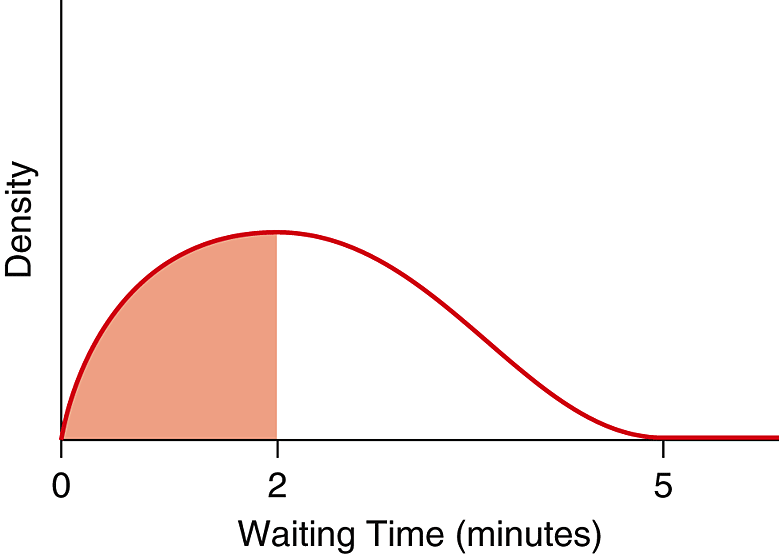
\includegraphics[width=0.4\linewidth]{images/math211_figure_6p6}
  \end{center}
  \vspace*{\stretch{1}}
  \pagebreak

  \begin{ex*}
    Suppose a bus arrives at the bus stop every 12 minutes. If you arrive at the bus stop at a randomly chosen time, then the probability distribution for the number of minutes you must wait is shown in the graph below:
  \end{ex*}
  \begin{center}
    \begin{tikzpicture}
      \begin{axis}[
        scaled ticks=false,
        /pgf/number format/.cd, fixed, precision=2, %forces large ytick labels
        axis x line=center,
        axis y line=left,
        axis line style={black,->},
        xmin=-1, xmax=13,
        ymin=0, ymax=0.125,
        enlargelimits={value=0.025, auto},
        ticklabel style={font=\footnotesize,inner sep=0.5pt,fill=white,opacity=1.0, text opacity=1},
        xlabel=Waiting Time (minutes), xlabel style={at={(axis description cs:0.5,-0.05)},anchor=north},
        ylabel=Density, ylabel style={at={(axis description cs:-0.1, 0.5)}, anchor=south},
        ]
        \addplot[draw=lander_blue, line width=1.25pt] (0,0) |- (12,1/12) -- (12,0);
      \end{axis}
    \end{tikzpicture}
  \end{center}
  
  \begin{extasks}[after-item-skip=\stretch{1}](1)
    \task Find the probability that you will have to wait less than 5 minutes.
    \task Find the probability that you will have to wait between 4 and 10 minutes.
    \task What is the probability that you will have to wait \emph{exactly} 12 minutes?
  \end{extasks}
  \vspace*{\stretch{0.5}}
  \pagebreak


  \pagebreak
\end{document}
